\documentclass[12pt, a4paper]{article}

\usepackage[utf8]{vietnam}
\usepackage{graphicx}
\usepackage{booktabs}
\usepackage{hyperref}
\usepackage{amsmath,amssymb}
\usepackage{enumitem}
\usepackage[top=2cm, bottom=2cm, left=2.5cm, right=2cm]{geometry}
\graphicspath{{bai2/}}

\begin{document}

\begin{center}
    {\Large \textbf{BÁO CÁO BÀI TẬP TUẦN 3}}
\end{center}

\section{Microbenchmark ngưỡng chuyển đổi PW sang SC (Bài 2)}

\textbf{Thí nghiệm lý thuyết.} Với clique kích thước $n$, số mệnh đề của hai cách mã hóa AMO là: pairwise $= \frac{n(n - 1)}{2}$ và sequential counter $= 3n - 4$. Giải bất phường trình $\frac{n(n - 1)}{2} > 3n - 4$, ta có $n > 5.56$, tức là từ $n \ge 6$, SC luôn ít mệnh đề hơn pairwise (tại $n = 6$: $14$ so với $15$; tại $n = 12$: $32$ so với $66$). Đây chính là cơ sở lý thuyết của ngưỡng $\theta = 6$ (Hình~\ref{fig:clause}).

\textbf{Thí nghiệm thực tế.} Với $n \in \{8, 10, 12, 15\}$, mỗi cấu hình lặp $200$ lần: sinh ngẫu nhiên một unit clause (đúng 1 biến = True), đo thời gian giải và thống kê của solver CaDiCaL153 (\texttt{solver.accum\_stats()}: conflicts, decisions, propagations). Kết quả (Hình~\ref{fig:runtime}): ở $n = 8$ hai mã hóa gần như ngang nhau (khác biệt trong nhiễu đo); từ $n \ge 10$ SC có xu hướng giảm conflicts và propagations so với pairwise. Kết luận thực nghiệm khớp với ngưỡng lý thuyết $\theta = 6$: với các clique nhỏ pairwise đủ tốt, SC chỉ có lợi khi clique lớn.

\begin{figure}[h!]
\centering
\begin{minipage}{0.48\textwidth}
    \centering
    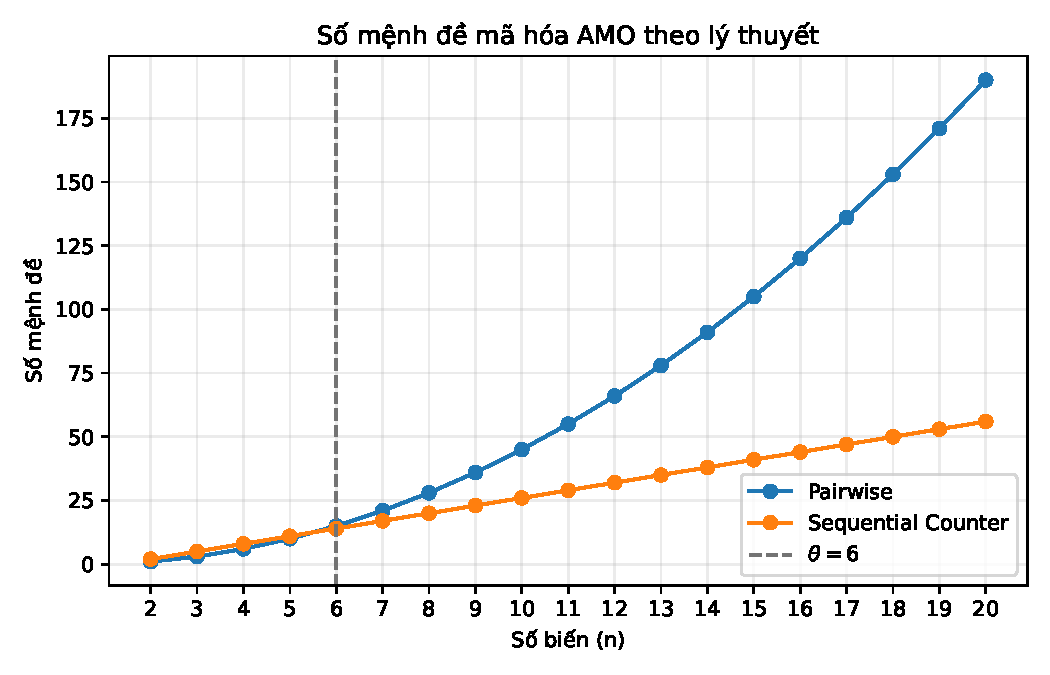
\includegraphics[width=\linewidth]{clause_count_comparison.pdf}
    \caption{Số mệnh đề lý thuyết.}
    \label{fig:clause}
\end{minipage}\hfill
\begin{minipage}{0.48\textwidth}
    \centering
    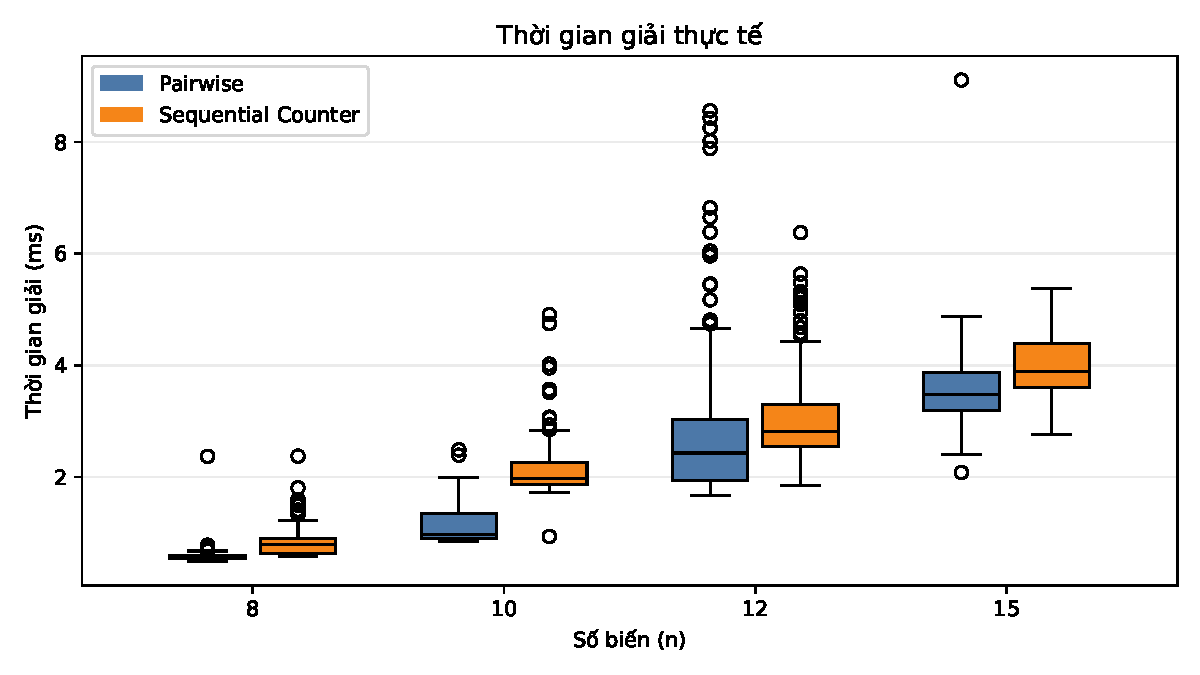
\includegraphics[width=\linewidth]{runtime_vs_n.pdf}
    \caption{Thời gian giải thực tế (CaDiCaL153, 200 lần lặp).}
    \label{fig:runtime}
\end{minipage}
\end{figure}

\section{Thống kê bộ benchmark 72 instances (Bài 3)}

Script \texttt{bai3\_instance\_stats.py} đọc toàn bộ 72 file instance (3 nhóm hạ tầng: \texttt{original}, \texttt{track}, \texttt{station}) và tính: số tàu, số operations, số cặp xung đột (cặp visit khác tàu cùng track), các thống kê clique, và tổng số time point ban đầu. Kết quả đầy đủ trong \\ \texttt{instance\_stats.csv} và \texttt{instance\_stats.tex}; bảng dưới tóm tắt các giá trị đại diện:

\begin{table}[htbp]
\centering
\resizebox{0.9\textwidth}{!}{%
\small
\begin{tabular}{lrrrrrrr}
\toprule
Instance & Trains & Ops & Conflicts & Cliques $\ge 6$ & Max clique & Mean clique & Initial TPs \\
\midrule
InstanceA1 (station) & 29 & 607 & 5915 & 0 & 2 & 2.00 & 1243 \\
InstanceA12 (station) & 28 & 608 & 6393 & 0 & 3 & 2.04 & 1244 \\
InstanceB2 (station) & 5 & 74 & 87 & 0 & 2 & 2.00 & 153 \\
InstanceB7 (orig) & 24 & 366 & 2865 & 0 & 4 & 2.50 & 756 \\
InstanceB11 (orig) & 25 & 385 & 3202 & 0 & 3 & 2.69 & 795 \\
\bottomrule
\end{tabular}%
}
\caption{Các instance đại diện}
\end{table}

\textbf{Nhận xét.} (i) Số time point ban đầu bằng số visit $= 2 \times \text{ops} + \text{trains}$, vì mỗi dòng track sinh 2 time variable (vào station và chạy trên track) cộng 1 biến đến ga đích cho mỗi tàu; giá trị này khớp với trường \texttt{avg\_time\_points} trong kết quả JSON của solver (A1: $1859 / 1.4955 \approx 1243$). (ii) Trên toàn bộ 72 instances, \textbf{không có clique nào có kích thước $\ge 6$} trong lịch gốc (max clique toàn bộ $= 4$, mean $\approx 2.0$--$2.7$). Điều này giải thích vì sao pairwise AMO là đủ, lợi thế của SC chỉ xuất hiện khi clique lớn hơn - đúng như cơ chế touched-clique AMO trong
solver.

\section{Đề xuất cải tiến formulation (Bài 4)}

\textbf{Câu 1: Ký hiệu thiếu định nghĩa tường minh.} Ba chỗ cần bổ sung vào đoạn
209-239: $H$ (planning horizon) được nêu nhưng không xuất hiện trong ràng buộc nào; $r_i^{\mathrm{dest}}$ (ga đích dùng trong công thức trễ $\delta_i$) chưa định nghĩa; các trọng số $w_{ik}, \eta_{ik}, w_i$ trong ba hàm chi phí không nói nguồn

\textbf{Câu 2: Separation bất đối xứng thành AMO clique.} Separation bất đối xứng được ``giấu'' vào cửa sổ unsafe, quyết định cặp indicator nào mutually incompatible tại $\tau$; các cặp đó tạo thành clique, và AMO trên clique tương đương hội các disjunction của các phần tử trong clique.

\textbf{Câu 3: Proposition exactness.} Đề xuất Mệnh đề gồm 2 khẳng định: (a) propagation: mọi lịch khả thi tự động thỏa các mệnh đề precedence mới (bound là hệ quả logic của ràng buộc đi đường, chứng minh quy nạp theo chuỗi chặng), nên không loại lịch nào; (b) SC equisatisfiable với pairwise AMO (theo Sinz 2005): cùng tập nghiệm, hàm mục tiêu không đổi nên cùng giá trị tối ưu;

\section{Sản phẩm}
\begin{itemize}
    \item \textbf{Bài 1}: \texttt{bai1/reviewer\_analysis.md}
    \item \textbf{Bài 2}: \texttt{bai2/bai2\_threshold\_sweep.py} +
          \texttt{clause\_count\_comparison.pdf} + \\ \texttt{runtime\_vs\_n.pdf}.
    \item \textbf{Bài 3}: \texttt{bai3/bai3\_instance\_stats.py} + \texttt{instance\_stats.csv} + \\ \texttt{instance\_stats.tex}.
    \item \textbf{Bài 4}: \texttt{bai4/reviewer\_proposal.md}.
    \item \textbf{Repository Git}:
          \url{https://github.com/Viing3107/maxsattrainscheduling/tree/tuan3_doquangvinh}
\end{itemize}

\end{document}